\subsubsection{\texttt{RF-9}: página de ayuda personalizada}
\label{subsec:rf9}

Uno de los objetivos de la presente evolución de \textit{VSCode4Teaching} es el de favorecer una mejor interacción entre los usuarios y la aplicación, haciéndola más intuitiva y fácil de usar, tal como establece el punto cuarto de los objetivos establecidos en el \referenciaCapitulo{cap:objetivos}.

En las versiones previas de \textit{VSCode4Teaching} se implementó un formato de inscripción en los cursos con el siguiente flujo de operaciones asociado: el profesor disponía de un botón para generar un código de invitación para estudiantes, quienes debían introducirlo en un cuadro de diálogo con su sesión abierta en la extensión para matricularse en el curso. Este proceso puede resultar complejo si se carece de una explicación adecuada previa.

En línea con el objetivo establecido, se ha aprovechado la introducción de la nueva aplicación web ---véase la \referenciaSeccion{sec:diseñoArquitectura} a este respecto--- para crear una página de ayuda nueva. De este modo, de ahora en adelante, el profesor genera un enlace de invitación a una página web (y no únicamente un código) que los estudiantes reciben y abren en su navegador web, donde pueden encontrar una página de ayuda como la que se refleja en la \referenciaFigura{fig:reqf9-1}. Esta página muestra una primera invitación que varía según el código introducido, reflejando el nombre del profesor y del curso al que se ha invitado al alumno, pudiendo así garantizar \textit{a priori} que se ha recibido el enlace de invitación correcto. A continuación, se introduce una serie de imágenes animadas que permiten a los estudiantes tener un primer acercamiento con el funcionamiento de \textit{VSCode4Teaching} y familiarizarse con las funcionalidades que tienen disponibles. Además, en el punto en que se explica cómo inscribirse al curso haciendo uso del código, disponen de un campo especial con un botón que les permite copiar al portapapeles este código fácilmente.

\begin{figure}[ht]
    \centering
    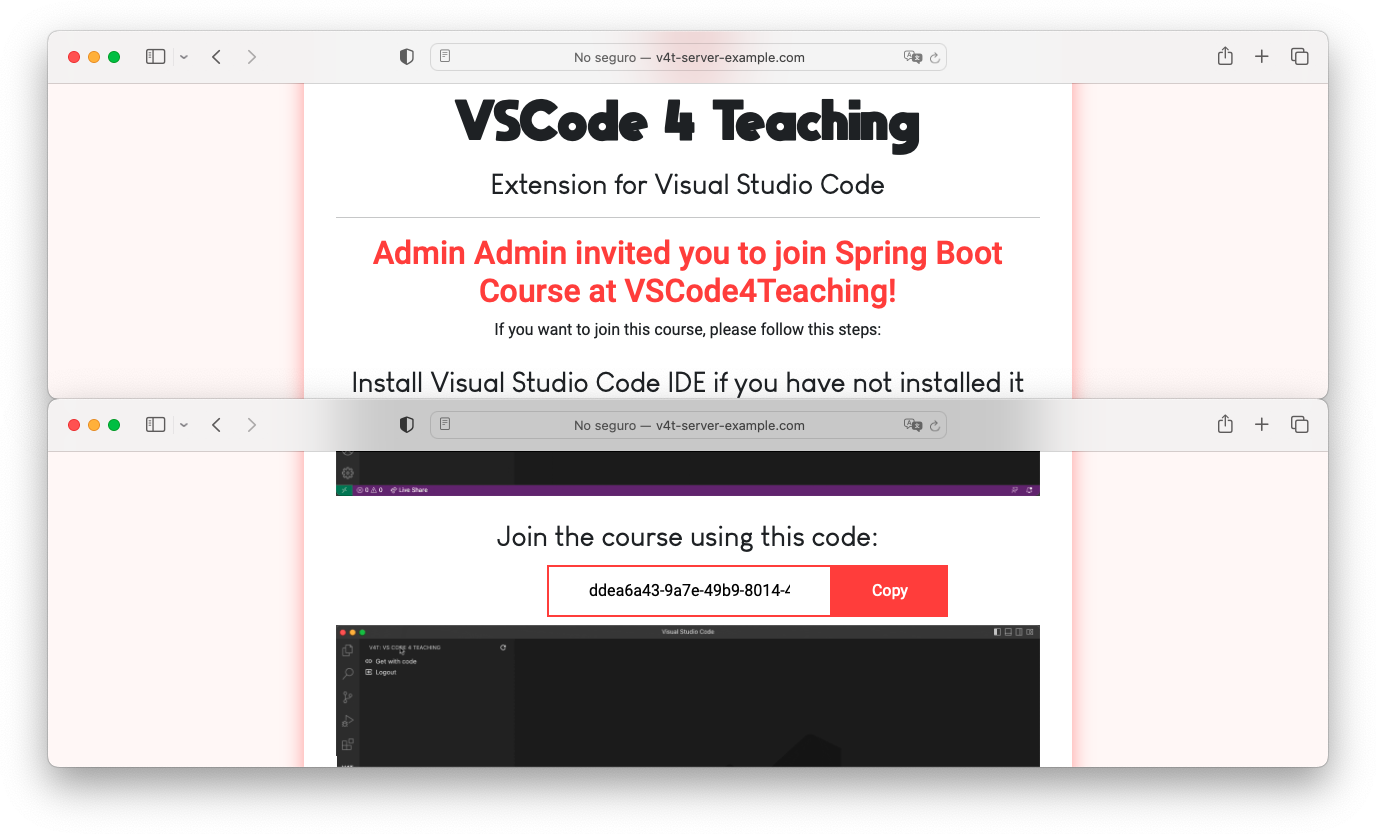
\includegraphics[width=\textwidth]{imagenes/utilizadas/4-3-implementacion/rf9-1.png}
    \caption{Captura de la página de ayuda personalizada según el código de invitación a curso suministrado.}
    \label{fig:reqf9-1}
\end{figure}
